% ! TeX root = ../../master-thesis.tex

\section{Stream Extension}
\label{section:implementation:stream-extension}

In support of the simulators and the test suite, the set of operations on
\texttt{Stream}s provided by Sodium has been extended with new operators for
the manipulation, analysis, and monitoring of \texttt{Stream}s. In designing
these operators, care was taken to preserve compositionality, implementing them
as pure functions, and fluency, integrating them into the existing
\texttt{Stream} class by means of Scala's \textit{extension methods}, also
because inheritance of the base types of \texttt{Sodium} is not allowed.

The collection of implemented extension methods is provided by the
\texttt{StreamEx\-tension} object, as illustrated in Figure
\ref{figure:stream-extension-class-diagram}.

\begin{figure}[!ht]
  \centering
  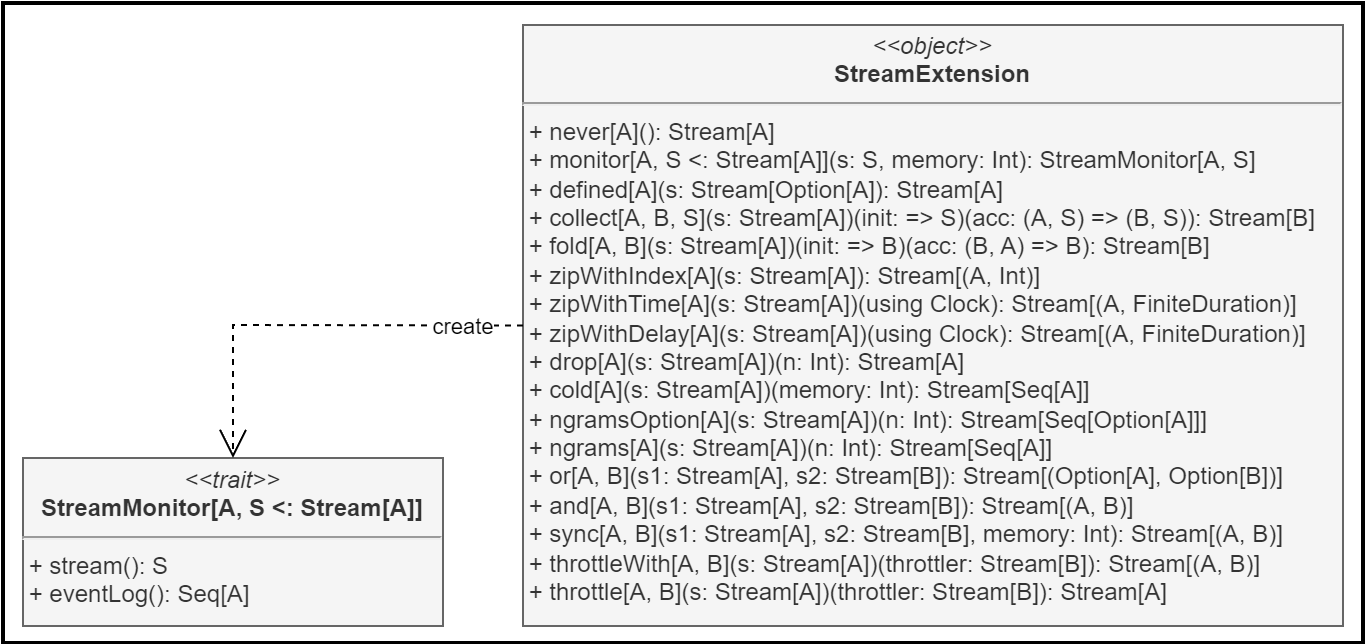
\includegraphics[width=0.8\textwidth]{resources/figures/stream-extension-class-diagram.png}
  \caption{
    A UML class diagram of the \texttt{Stream} extension
    and its operators.
  }
  \label{figure:stream-extension-class-diagram}
\end{figure}

\subsection{Persistence Operators}

The following operators can be used to deal with state persistence in
\texttt{Stream}s:

\begin{itemize}
  \item \texttt{collect}: evolve an initial state \texttt{init} as the
        input \texttt{Stream} $s$ generates new events and return an output
        \texttt{Stream} $s'$, whose events are a combination of the events
        fired by $s$ with the current state at the moment of firing. The
        \texttt{acc} function defines both the evolution of the state and the
        events of $s'$ depending on the firings of $s$.

        The \texttt{collect} operator is an adaptation for Scala of the
        homonymous operator provided by \texttt{Sodium} in Java.

  \item \texttt{fold}: a simplification of the \texttt{collect}
        operator, in which the events of the output \texttt{Stream} $s'$ are a
        snapshot of the current state taken at each firing of the input
        \texttt{Stream} $s$. The \texttt{acc} function defines the evolution of
        the state depending on the firings of $s$, and the events of $s'$ as a
        consequence.

        The \texttt{fold} operator is an implementation of the \textit{folding}
        operation provided by Scala for all \texttt{Iterable}s. However, the
        events of the input \texttt{Stream} are folded lazily as they are
        fired.
\end{itemize}

An example of their application is the evolution of the global view of an
aggregate, such as the method \texttt{exportedByAll}, obtained by accumulating
the individual device exports generated during a simulation.

\subsection{Temporal Operators}

The following operators can be used to perform time-sensitive analysis on
\texttt{Stream}s:

\begin{itemize}
  \item \texttt{zipWithIndex}: when applied to an input \texttt{Stream} $s$,
        return an output \texttt{Stream} $s'$, whose events are the same events
        of $s$ paired with the discrete time when they were fired. Discrete
        time is modelled as the number of firings preceding an event in $s$.
  \item \texttt{zipWithTime}: when applied to a \texttt{Stream} $s$, return an
        output \texttt{Stream} $s'$, whose events are the same events of $s$
        paired with the continuous time when they were fired. Continuous time
        is defined by a given \texttt{Clock}, which defaults to the number of
        nanoseconds elapsed since the creation of $s'$. Abstracting over
        real-world time allows the user to provide their own implementation of
        \texttt{Clock} to achieve complete control on the timeline of the
        \texttt{Stream}, which can be useful to avoid non-determinism during
        tests.
  \item \texttt{zipWithDelay}: when applied to an input \texttt{Stream} $s$,
        return an output \texttt{Stream} $s'$, whose events are the same events
        of $s$ paired with the continuous time elapsed since the previous
        event. Similarly to \texttt{zipWithTime}, continuous time is defined by
        a given \texttt{Clock}.
\end{itemize}

An example of their application is the implementation of time-sensitive
\texttt{Halt\-Policy}s, such as the \texttt{haltAfter} policy, introduced in
Section \ref{section:implementation:step-simulator}.

\subsection{Derivation Operators}

The following operators can be used to perform trend and behaviour analysis on
\texttt{Stream}s:

\begin{itemize}
  \item \texttt{ngrams}: when applied to an input \texttt{Stream} $s$, return
        an output \texttt{Stream} $s'$, whose events are all the possible
        groups of consecutive events fired by $s$ with cardinality $n$. Note
        that $s'$ does not fire any event until $s$ has emitted at least $n$
        events, which may never happen. In such case, any information about the
        events of $s$ is lost in $s'$.
  \item \texttt{ngramsOption}: as \texttt{ngrams}, but information loss is
        prevented by producing incomplete groups in $s'$ until $s$ has
        generated at least $n$ events. An incomplete group contains all the
        consecutive events fired by $s$ and as many placeholder values needed
        to reach cardinality $n$. In particular, \texttt{Option.None} is used
        as a placeholder value.
\end{itemize}

A future application of these operators could be the verification of more
sophisticated temporal properties against the evolution of aggregates, checking
the behaviour of the aggregate during a fixed time-window (e.g., evaluating if
the sum of the outputs of all the devices is always the sum at the previous
step plus one).

\subsection{Monitoring Operators}

The following operators can be used to monitor the events generated by
\texttt{Stream}s:
\begin{itemize}
  \item \texttt{cold}: when applied to an input \texttt{Stream} $s$, return an
        output \texttt{Stream} $s'$, whose events are sequences containing all
        the firings of $s$ after the creation of $s'$. Since $s$ may fire
        events indefinitely, the length of the sequences can be limited to a
        given amount of \texttt{memory}, which corresponds to the number of
        events of $s$ kept in memory by the operator. When the memory is full,
        the oldest events are replaced with the newest ones as they are fired.

        The name of this operator comes from the notion of \textbf{cold
        observable}s, as described in Section 6.2.1 of the book \cite{FRP}. In
        Sodium, all \texttt{Stream}s are inherently \textbf{hot observable}s,
        meaning that any dependent will react only to the events that are fired
        after its dependency has been declared, ignoring all the events that
        were fired before. The \texttt{cold} operator creates a \texttt{Stream}
        that acts \textit{almost} as a cold observable variant of the original
        \texttt{Stream}, by letting the dependents react also to the events
        that were fired before the declaration of their dependencies. However,
        dependents will be notified of all the events of the original
        \texttt{Stream} only after its next firing, which may never happen. To
        solve this problem, the \texttt{Stream} can be transformed into a
        \texttt{Cell} by means of the \texttt{hold} operator, obtaining an
        actual cold observable. In fact, \texttt{Cell}s propagate their latest
        state as soon as a dependent is declared.

  \item \texttt{monitor}: when applied to an input \texttt{Stream} $s$, return
        a \texttt{StreamMonitor} wrapping $s$. A \texttt{StreamMonitor} relies
        on the \texttt{cold} operator to monitor the wrapped \texttt{Stream},
        exposing a sequence of all its events, accessible at any time by means
        of the method \texttt{eventLog}. In other words, a
        \texttt{StreamMonitor} converts a \texttt{Stream} into an up-to-date
        list of its events. Similarly to the \texttt{cold} operator, the length
        of the sequence can be limited to reduce memory costs.
\end{itemize}

The purpose of these operators is to decouple the generation of the events of a
\texttt{Stream} from the evaluation of their properties, which greatly
simplifies testing. However, performing the evaluation during the generation of
the events would be more efficient, as the program generating the events could
be interrupted prematurely if the property was already proven before the
program termination. Naturally, this optimization cannot be implemented by
leveraging these operators, since the evaluation starts only after the program
termination.

An example of their application is the implementation of most of the test suite
and the \texttt{ConvergenceSim\-ulator}, in which the global view of the
aggregate is monitored to return its latest state when the simulation is
halted.

\subsection{Throttling Operators}

The following operators can be used to control the throughput of
\texttt{Stream}s:
\begin{itemize}
  \item \texttt{sync}: combine two input \texttt{Stream}s $s_1$ and $s_2$,
        returning an output \texttt{Stream} $s'$, whose events are the pairs of
        corresponding events in $s_1$ and $s_2$. More formally, the $k^{th}$
        event of $s'$ is a pair containing the $k^{th}$ event of $s_1$ and the
        $k^{th}$ event of $s_2$. Since $s_1$ and $s_2$ may fire their $k^{th}$
        event at different times, the operator requires keeping in memory the
        latest unpaired events of both \texttt{Stream}s. Similarly to the
        \texttt{cold} and \texttt{monitor} operators, the number of events
        stored for each \texttt{Stream} can be limited to a given
        \texttt{memory}.

        An implication of the \texttt{sync} operator is that the throughput of
        the output \texttt{Stream} is equal to the lowest throughput between
        the input \texttt{Stream}s, meaning that the operator can be used to
        control the frequency at which a \texttt{Stream} emits its events.
        Additionally, by limiting the memory of the operator, some events of
        the \texttt{Stream} with the highest throughput may be discarded when
        the memory is full, preventing possible overloads of its dependents.
  \item \texttt{throttleWith}: a specialization of the \texttt{sync} operator
        with unitary \texttt{memory}, storing only the latest unpaired event of
        each input \texttt{Stream}.
  \item \texttt{throttle}: a specialization of the \texttt{throttleWith}
        operator, in which the output \texttt{Stream} $s'$ fires the events of
        the first input \texttt{Stream} $s_1$, while the second input
        \texttt{Stream} $s_2$ acts only as a throttle for $s_1$.
\end{itemize}

A future application of these operators could be regulating the event
production rate of reactive variables in general, including \texttt{Stream}s,
\texttt{Cell}s and possibly \texttt{Flow}s.
